\section{光滑化}
\label{sec:ns-smoothing}

邻近方法要求非光滑项的邻近映射便宜。有限个仿射函数的最大值常常做不到这一点：它的邻近子问题本身是一个二次规划。于是要问：能否把尖点磨圆，得到一个光滑的替代目标，再调用第~\ref{chap:first-order-methods}章的方法，并算清这样做对原问题到底造成多大误差？

光滑化改变的是目标，第~\ref{chap:first-order-methods}章的Nesterov加速改变的是迭代规则，这是两件独立的事，后面会把它们配合使用。从本节起，$\mu>0$表示平滑参数，$\mu$越小替代目标越接近原目标。

\subsection{Huber逼近}
\label{sec:ns-huber}

最简单的尖点是$\lvert x\rvert$的原点。把原点两侧长度为$\mu$的两段折线换成一段抛物线，外面保持直线，就把尖点磨掉了。外面的直线不能是$\lvert x\rvert$本身，否则接不上，要向下平移一段。设抛物线是$x^2/(2\mu)$，外侧是$\lvert x\rvert-c$，在接点$x=\mu$处要求函数值和一阶导数都匹配。

一阶导数：抛物线的导数是$x/\mu$，在$x=\mu$处等于$1$，正好等于外侧直线的斜率，这是抛物线取系数$1/(2\mu)$的原因。

函数值：抛物线在接点的值是$\mu/2$，要求$\mu-c=\mu/2$，所以$c=\mu/2$。

这样得到\term{Huber函数}（Huber function）\scite{huber1964}
\begin{equation}
 h_\mu(x)=\begin{cases}
 \dfrac{x^2}{2\mu},&\lvert x\rvert\leq\mu,\\
 \lvert x\rvert-\dfrac{\mu}{2},&\lvert x\rvert>\mu.
 \end{cases}
 \label{eq:ns-huber}
\end{equation}

下面的性质说明它是一个可控的替代。

\begin{theorem}[Huber逼近的性质]
\label{thm:ns-huber}
对任意$\mu>0$，$h_\mu$是连续可微的凸函数，并且
\begin{gather}
 0\leq\lvert x\rvert-h_\mu(x)\leq\frac{\mu}{2},\label{eq:ns-huber-gap}\\
 h_\mu'(x)=\min\Bigl\{\max\Bigl\{\frac{x}{\mu},\,-1\Bigr\},\,1\Bigr\},\qquad
 \lvert h_\mu'(x)-h_\mu'(y)\rvert\leq\frac{1}{\mu}\lvert x-y\rvert.\label{eq:ns-huber-grad}
\end{gather}
\end{theorem}

\begin{proof}
由接点匹配，$h_\mu$在$\pm\mu$处连续可微，其余点是二次函数或线性函数，也可微，导数就是式~\eqref{eq:ns-huber-grad}。这个导数是$x/\mu$截断到$[-1,1]$，它单调不减（所以$h_\mu$凸）。截断不增大距离，而$x/\mu$的Lipschitz常数是$1/\mu$，所以导数$1/\mu$-Lipschitz。

偏差只需看$x\geq0$。外侧$\lvert x\rvert-h_\mu(x)=\mu/2$。内侧令$e(x)=x-x^2/(2\mu)$，$e(0)=0$，$e'(x)=1-x/\mu\geq0$，所以$e$从$0$单调增到$e(\mu)=\mu/2$。
\end{proof}

图~\ref{fig:ns-huber}画出两个$\mu$。(a)中$h_\mu$从下方逼近$\lvert x\rvert$，$\mu$减半时差也减半。(b)中$\lvert x\rvert$的导数在原点跳变，$h_\mu'$用一段斜率$1/\mu$的直线走完这段跳变。$\mu$减半，过渡段的斜率加倍，这就是梯度Lipschitz常数$1/\mu$的来源。

\begin{BookInlineFigure}
  \centering
  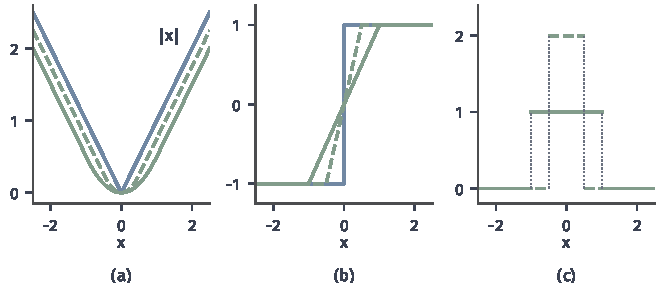
\includegraphics[width=112mm]{figures/05-optimization/03-nonsmooth-optimization/matplotlib/ns-huber/figure.pdf}
  \caption{Huber函数。蓝线是$\lvert x\rvert$及其导数，绿色实线和虚线分别是$\mu=1$和$\mu=\tfrac12$的$h_\mu$。(a)函数值，$h_\mu$在外侧与$\lvert x\rvert$平行。(b)一阶导数，连续但有拐点。(c)二阶导数，在接点$\pm\mu$处跳变，所以$h_\mu$在这些点不是二阶可微的。}
  \label{fig:ns-huber}
\end{BookInlineFigure}

要留意图~\ref{fig:ns-huber}(c)。$h_\mu$的二阶导数在$\lvert x\rvert<\mu$处是$1/\mu$，在外面是$0$，在接点上不存在。所以$h_\mu$的梯度Lipschitz，但不是处处二阶可微。第~\ref{chap:smooth-foundations}章的一阶方法只需要前者，可以直接用；第~\ref{chap:second-order-methods}章的牛顿法在接点附近没有定义好的Hessian，要专门处理。

\subsection{Moreau包络}
\label{sec:ns-moreau}

Huber函数的抛物线从何而来？它其实是第~\ref{sec:ns-proximal}节的邻近子问题的副产品：邻近映射取的是最小点，如果取最优值，就得到一个新函数。

\begin{definition}[Moreau包络]
\label{def:ns-moreau}
设$f$是适当、下半连续的凸函数，$\mu>0$。称
\begin{equation}
 M_{\mu f}(\bm{x})=\min_{\bm{y}}\Bigl\{f(\bm{y})+\frac{1}{2\mu}\lVert\bm{y}-\bm{x}\rVert_2^2\Bigr\}
 \label{eq:ns-moreau}
\end{equation}
为$f$的\term{Moreau包络}（Moreau envelope）。
\end{definition}

由定理~\ref{thm:ns-prox}，最小值在唯一的$\bm{p}=\operatorname{prox}_{\mu f}(\bm{x})$处取到，所以$M_{\mu f}$处处有限。

对$f=\lvert\cdot\rvert$用软阈值计算。若$\lvert x\rvert\leq\mu$，$p=0$，结果是$x^2/(2\mu)$。若$\lvert x\rvert>\mu$，$p=x-\mu\operatorname{sign}(x)$，$\lvert p\rvert=\lvert x\rvert-\mu$，距离项是$\mu/2$，结果是$\lvert x\rvert-\mu/2$。两种情形合起来正是式~\eqref{eq:ns-huber}：
\begin{equation}
 M_{\mu\lvert\cdot\rvert}=h_\mu.
 \label{eq:ns-moreau-huber}
\end{equation}

这个包络的图景是：把一个以$\bm{x}$为顶点的小抛物线碗从下往上抬，碰到$f$时碗顶的高度就是$M_{\mu f}(\bm{x})$。图~\ref{fig:ns-moreau-envelope}(a)画出了三段折线的包络，折点都被抛物线磨圆。

\begin{theorem}[Moreau包络的光滑性与最小点]
\label{thm:ns-moreau}
设$f$是适当、下半连续的凸函数，$\mu>0$。则$M_{\mu f}$是凸函数，处处可微，且
\begin{equation}
 \nabla M_{\mu f}(\bm{x})=\frac{\bm{x}-\operatorname{prox}_{\mu f}(\bm{x})}{\mu}.
 \label{eq:ns-moreau-grad}
\end{equation}
梯度是$1/\mu$-Lipschitz的。此外$M_{\mu f}\leq f$，并且$M_{\mu f}$与$f$有相同的最小值和相同的最小点集合。
\end{theorem}

\begin{proof}
记$\bm{p}=\operatorname{prox}_{\mu f}(\bm{x})$，$\bm{s}=(\bm{x}-\bm{p})/\mu$，由式~\eqref{eq:ns-prox-characterization}有$\bm{s}\in\partial f(\bm{p})$。任取$\bm{y}$，记$\bm{q}=\operatorname{prox}_{\mu f}(\bm{y})$。

上界。把$\bm{p}$作为$\bm{y}$处子问题的试探点，
\[
 M_{\mu f}(\bm{y})\leq f(\bm{p})+\frac{1}{2\mu}\lVert\bm{p}-\bm{y}\rVert_2^2=M_{\mu f}(\bm{x})+\langle\bm{s},\bm{y}-\bm{x}\rangle+\frac{1}{2\mu}\lVert\bm{y}-\bm{x}\rVert_2^2.
\]
第二个等号是把$\bm{p}-\bm{y}=(\bm{p}-\bm{x})+(\bm{x}-\bm{y})$展开，并用$\bm{p}-\bm{x}=-\mu\bm{s}$。

下界。由$\bm{s}\in\partial f(\bm{p})$，
\[
 f(\bm{q})\geq f(\bm{p})+\langle\bm{s},\bm{q}-\bm{p}\rangle,
\]
于是
\[
 M_{\mu f}(\bm{y})-M_{\mu f}(\bm{x})\geq\langle\bm{s},\bm{q}-\bm{p}\rangle+\frac{1}{2\mu}\Bigl(\lVert\bm{q}-\bm{y}\rVert_2^2-\lVert\bm{p}-\bm{x}\rVert_2^2\Bigr).
\]

记$\bm{a}=\bm{q}-\bm{y}$，$\bm{b}=\bm{p}-\bm{x}=-\mu\bm{s}$，再用恒等式
\[
 \lVert\bm{a}\rVert_2^2-\lVert\bm{b}\rVert_2^2=\lVert\bm{a}-\bm{b}\rVert_2^2+2\langle\bm{a}-\bm{b},\bm{b}\rangle,
\]
右端化为
\[
 \langle\bm{s},\bm{y}-\bm{x}\rangle+\frac{1}{2\mu}\lVert\bm{a}-\bm{b}\rVert_2^2\geq\langle\bm{s},\bm{y}-\bm{x}\rangle.
\]

上下界合起来，
\[
 0\leq M_{\mu f}(\bm{y})-M_{\mu f}(\bm{x})-\langle\bm{s},\bm{y}-\bm{x}\rangle\leq\frac{1}{2\mu}\lVert\bm{y}-\bm{x}\rVert_2^2.
\]
所以$M_{\mu f}$在$\bm{x}$处可微，梯度为$\bm{s}$。下界对所有$\bm{x}$成立，说明处处存在次梯度，因而是凸函数。

Lipschitz性。记$\bm{u}=\bm{x}-\bm{y}$，$\bm{w}=\bm{p}-\bm{q}$，由式~\eqref{eq:ns-firm-nonexpansive}得$\lVert\bm{w}\rVert_2^2$不超过$\langle\bm{u},\bm{w}\rangle$，所以
\[
 \lVert\bm{u}-\bm{w}\rVert_2^2=\lVert\bm{u}\rVert_2^2-2\langle\bm{u},\bm{w}\rangle+\lVert\bm{w}\rVert_2^2\leq\lVert\bm{u}\rVert_2^2-\lVert\bm{w}\rVert_2^2\leq\lVert\bm{u}\rVert_2^2.
\]
梯度之差是$(\bm{u}-\bm{w})/\mu$，范数不超过$\lVert\bm{u}\rVert_2/\mu$。

最小点。在式~\eqref{eq:ns-moreau}中取$\bm{y}=\bm{x}$得$M_{\mu f}\leq f$。$\bm{x}$是$M_{\mu f}$的最小点，当且仅当梯度为零，当且仅当$\bm{x}=\operatorname{prox}_{\mu f}(\bm{x})$，由式~\eqref{eq:ns-prox-characterization}当且仅当$\bm{0}\in\partial f(\bm{x})$。此时距离项为零，$M_{\mu f}(\bm{x})=f(\bm{x})$，所以最小值相同。
\end{proof}

对$\lvert x\rvert$验证式~\eqref{eq:ns-moreau-grad}。$x=2$，$\mu=1$时$p=1$，公式给出$(2-1)/1=1$，这就是Huber函数在外侧的斜率。$x=0.6$时$p=0$，公式给出$0.6$，与$h_1'(0.6)=0.6$一致。

\paragraph{平滑一项不等于保持解}
定理说整个凸目标的包络与原函数有相同的最小点。但实用上想平滑的通常只是复合目标的一项。这时最小点一般会变。

取$F(x)=\tfrac12(x-\tfrac12)^2+\lvert x\rvert$。在$x=0$处$F$的次微分是$-\tfrac12+[-1,1]$，包含零，所以$x^\star=0$。只把$\lvert x\rvert$换成包络$h_1$，得到光滑目标$F_1(x)=\tfrac12(x-\tfrac12)^2+h_1(x)$，在$\lvert x\rvert\leq1$上令导数为零：
\[
 x-\frac12+x=0,\qquad x=\frac14.
\]

原问题的解是$0$，这个替代的解是$\tfrac14$。图~\ref{fig:ns-moreau-envelope}(b)显示了这一点。代入原目标，$F(\tfrac14)=\tfrac{9}{32}\approx0.281$，比$F^\star=\tfrac18$高，$\tfrac14$不再有“稀疏”的零分量。

\begin{BookInlineFigure}
  \centering
  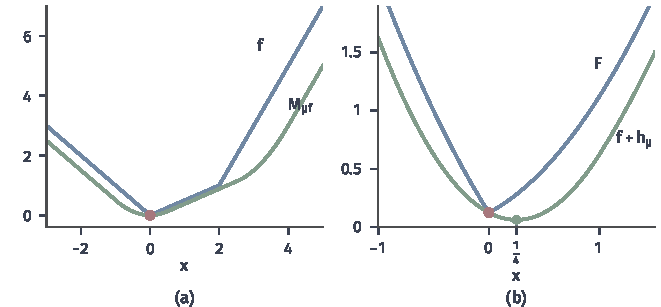
\includegraphics[width=112mm]{figures/05-optimization/03-nonsmooth-optimization/matplotlib/ns-moreau-envelope/figure.pdf}
  \caption{Moreau包络（$\mu=1$）。(a)三段折线$f$（蓝）与它的包络（绿），最小点相同（红点）。(b)$F(x)=\tfrac12(x-\tfrac12)^2+\lvert x\rvert$（蓝）的最小点是$0$（红点），只平滑绝对值项后，绿色替代目标的最小点移到$\tfrac14$（绿点）。}
  \label{fig:ns-moreau-envelope}
\end{BookInlineFigure}

求包络的梯度~\eqref{eq:ns-moreau-grad}要算一次邻近映射。所以包络不能绕开邻近映射：当$\operatorname{prox}$不便宜时，这条路同样走不通。这正是下面的方法要解决的问题。

\subsection{Nesterov平滑}
\label{sec:ns-nesterov-smoothing}

许多非光滑函数天然写成最大值，比如分段线性函数和$\ell_1$范数。最大值函数的梯度在活跃分支切换时跳变。Nesterov平滑的想法是让这种切换变得连续，方法是在最大化问题的变量上加入一点强凸惩罚，使每个$\bm{x}$对应唯一的内层最优点，而这个最优点随$\bm{x}$连续变化。

\subsubsection{最大值表示的正则化}
\label{sec:ns-max-regularization}

设目标有最大值结构：$\bm{A}\in\mathbb{R}^{p\times n}$，$\bm{Q}\subset\mathbb{R}^p$是非空紧凸集，$\phi$是$\bm{Q}$上的连续凸函数，
\begin{equation}
 f(\bm{x})=\max_{\bm{u}\in\bm{Q}}\bigl\{\langle\bm{A}\bm{x},\bm{u}\rangle-\phi(\bm{u})\bigr\}.
 \label{eq:ns-max-form}
\end{equation}

例如$\lvert x\rvert=\max_{\lvert u\rvert\leq1}xu$，最优的$u$是$\operatorname{sign}(x)$，在$x=0$处从$-1$跳到$1$，这就是梯度的跳变。

在$\bm{u}$的空间选一个范数$\lVert\cdot\rVert_{\bm{Q}}$。设$d:\bm{Q}\to\mathbb{R}$连续，$\sigma$-强凸（对这个范数），且$\min_{\bm{Q}}d=0$。记$D=\max_{\bm{Q}}d$，矩阵的范数
\[
 \lVert\bm{A}\rVert=\max\bigl\{\langle\bm{A}\bm{x},\bm{u}\rangle:\ \lVert\bm{x}\rVert_2\leq1,\ \lVert\bm{u}\rVert_{\bm{Q}}\leq1\bigr\}.
\]

这里的$\sigma$-强凸是指对$\bm{u},\bm{v}\in\bm{Q}$，$\theta\in[0,1]$，
\begin{equation}
 d\bigl(\theta\bm{u}+(1-\theta)\bm{v}\bigr)\leq\theta d(\bm{u})+(1-\theta)d(\bm{v})-\frac{\sigma}{2}\theta(1-\theta)\lVert\bm{u}-\bm{v}\rVert_{\bm{Q}}^2.
 \label{eq:ns-sigma-strong}
\end{equation}
在最大化式里减去$\mu d$，定义\term{Nesterov平滑}（Nesterov smoothing）
\begin{equation}
 f_\mu(\bm{x})=\max_{\bm{u}\in\bm{Q}}\bigl\{\langle\bm{A}\bm{x},\bm{u}\rangle-\phi(\bm{u})-\mu d(\bm{u})\bigr\}.
 \label{eq:ns-nesterov}
\end{equation}

\begin{theorem}[Nesterov平滑的性质]
\label{thm:ns-nesterov}
在上述条件下，式~\eqref{eq:ns-nesterov}对每个$\bm{x}$有唯一的最大点，记作$\bm{u}_\mu(\bm{x})$。函数$f_\mu$凸且可微，并且
\begin{gather}
 \nabla f_\mu(\bm{x})=\bm{A}^\top\bm{u}_\mu(\bm{x}),\label{eq:ns-nesterov-grad}\\
 f_\mu(\bm{x})\leq f(\bm{x})\leq f_\mu(\bm{x})+\mu D,\label{eq:ns-nesterov-gap}\\
 \lVert\nabla f_\mu(\bm{x})-\nabla f_\mu(\bm{y})\rVert_2\leq\frac{\lVert\bm{A}\rVert^2}{\mu\sigma}\lVert\bm{x}-\bm{y}\rVert_2.\label{eq:ns-nesterov-lip}
\end{gather}
\end{theorem}

\begin{proof}
记式~\eqref{eq:ns-nesterov}中大括号内的函数为$\Psi_{\bm{x}}(\bm{u})$。$\phi$是凸的，$\mu d$是$\mu\sigma$-强凸的，所以$\Psi_{\bm{x}}$是$\mu\sigma$-强凹的连续函数，在紧凸集上有唯一的最大点。

强凹性给出最大点处的二次间隙。设$\bm{u}_1$是最大点，对任意$\bm{u}\in\bm{Q}$和$\theta\in(0,1)$，令$\bm{w}=\theta\bm{u}+(1-\theta)\bm{u}_1\in\bm{Q}$，
\[
 \Psi_{\bm{x}}(\bm{u}_1)\geq\Psi_{\bm{x}}(\bm{w})\geq\theta\Psi_{\bm{x}}(\bm{u})+(1-\theta)\Psi_{\bm{x}}(\bm{u}_1)+\frac{\mu\sigma}{2}\theta(1-\theta)\lVert\bm{u}-\bm{u}_1\rVert_{\bm{Q}}^2.
\]

整理后除以$\theta$，再令$\theta\to0$，得到
\begin{equation}
 \Psi_{\bm{x}}(\bm{u})\leq\Psi_{\bm{x}}(\bm{u}_1)-\frac{\mu\sigma}{2}\lVert\bm{u}-\bm{u}_1\rVert_{\bm{Q}}^2.
 \label{eq:ns-strong-concave-gap}
\end{equation}

Lipschitz估计。对$\bm{x}_1,\bm{x}_2$，记$\bm{u}_i=\bm{u}_\mu(\bm{x}_i)$。式~\eqref{eq:ns-strong-concave-gap}两次使用后相加，$\phi$和$d$的项消去，得到
\[
 \mu\sigma\lVert\bm{u}_1-\bm{u}_2\rVert_{\bm{Q}}^2\leq\langle\bm{A}(\bm{x}_1-\bm{x}_2),\bm{u}_1-\bm{u}_2\rangle\leq\lVert\bm{A}\rVert\,\lVert\bm{x}_1-\bm{x}_2\rVert_2\,\lVert\bm{u}_1-\bm{u}_2\rVert_{\bm{Q}}.
\]

约去一个$\lVert\bm{u}_1-\bm{u}_2\rVert_{\bm{Q}}$，得到
\[
 \lVert\bm{u}_1-\bm{u}_2\rVert_{\bm{Q}}\leq\frac{\lVert\bm{A}\rVert}{\mu\sigma}\lVert\bm{x}_1-\bm{x}_2\rVert_2.
\]

梯度公式。$f_\mu$是一族仿射函数的上确界，所以是凸的。取$\bm{u}=\bm{u}_\mu(\bm{x})$，$\bm{u}'=\bm{u}_\mu(\bm{y})$，一方面
\[
 f_\mu(\bm{y})\geq\Psi_{\bm{y}}(\bm{u})=f_\mu(\bm{x})+\langle\bm{A}^\top\bm{u},\bm{y}-\bm{x}\rangle.
\]

另一方面，由$\Psi_{\bm{x}}(\bm{u}')\leq f_\mu(\bm{x})$，
\[
 f_\mu(\bm{y})=\Psi_{\bm{y}}(\bm{u}')\leq f_\mu(\bm{x})+\langle\bm{A}^\top\bm{u},\bm{y}-\bm{x}\rangle+\langle\bm{A}(\bm{y}-\bm{x}),\bm{u}'-\bm{u}\rangle.
\]
由上一段的估计，最后一项不超过$\lVert\bm{A}\rVert^2\lVert\bm{y}-\bm{x}\rVert_2^2/(\mu\sigma)$，是二阶小量，所以$f_\mu$可微，梯度是$\bm{A}^\top\bm{u}$。

式~\eqref{eq:ns-nesterov-lip}由上面的估计和下面的范数关系得到：
\[
 \lVert\bm{A}^\top(\bm{u}_1-\bm{u}_2)\rVert_2\leq\lVert\bm{A}\rVert\,\lVert\bm{u}_1-\bm{u}_2\rVert_{\bm{Q}}.
\]

偏差。由$0\leq d\leq D$，对每个$\bm{u}$有
\[
 \langle\bm{A}\bm{x},\bm{u}\rangle-\phi(\bm{u})-\mu D\leq\Psi_{\bm{x}}(\bm{u})\leq\langle\bm{A}\bm{x},\bm{u}\rangle-\phi(\bm{u}).
\]
对$\bm{u}$取最大，就是式~\eqref{eq:ns-nesterov-gap}。
\end{proof}

每个条件的作用都清楚：紧性使$D$有限，从而偏差有限；强凸使内层解唯一且随$\bm{x}$连续变化，梯度跳变由此被抹平；$\min d=0$让偏差是单侧的。$\mu$变小时偏差$\mu D$变小，Lipschitz常数$\lVert\bm{A}\rVert^2/(\mu\sigma)$变大，后面就是要权衡这两者。

用菱形目标算一遍。写成$\bm{A}=\operatorname{diag}(1,2)$，$\bm{Q}=[-1,1]^2$，$\phi=0$，$d(\bm{u})=\tfrac12\lVert\bm{u}\rVert_2^2$，$\sigma=1$，范数取欧氏范数。此时$D=1$，$\lVert\bm{A}\rVert=2$。内层问题按坐标分开，解是把$(\bm{A}\bm{x})_i/\mu$截断到$[-1,1]$，把解代回，得到
\[
 f_\mu(\bm{x})=h_\mu(x_1)+h_\mu(2x_2),\qquad\nabla f_\mu(\bm{x})=\bm{A}^\top\bm{u}_\mu(\bm{x}).
\]

结果是两个Huber函数之和，第二项的二阶导数最大为$4/\mu$，正好是$\lVert\bm{A}\rVert^2/(\mu\sigma)$。在$\bm{x}=(1,0)$，$\mu=1$处，
\[
 \bm{u}_1=(1,0),\qquad f_1(\bm{x})=\frac12,\qquad f(\bm{x})-f_1(\bm{x})=\frac12\leq\mu D=1.
\]

内层求解的成本决定这个方法是否划算。本例内层是逐坐标截断，$O(n)$；$\bm{Q}$是单纯形且$d$取下面的负熵时也是闭式解。若$\bm{Q}$或$\phi$没有这样的结构，每次读梯度都要解一个内层优化，只能得到近似的$\bm{u}_\mu$，这时梯度带有误差，上面的保证需要重新计入这个误差。

\subsubsection{对数和指数平滑}
\label{sec:ns-log-sum-exp}

最常用的实例是有限个仿射函数的最大值，也就是开头提到的邻近映射不便宜的情形。设$\ell_i(\bm{x})=\langle\bm{a}_i,\bm{x}\rangle+b_i$，$i=1,\ldots,m$，这里$m$是分支个数。

把“选一个最大的分支”写成单纯形$\Delta_m=\{\bm{u}\geq\bm{0}:\sum_iu_i=1\}$上的线性最大化，权重集中在最大的分支上时取到最大值：
\[
 f(\bm{x})=\max_i\ell_i(\bm{x})=\max_{\bm{u}\in\Delta_m}\sum_{i=1}^mu_i\ell_i(\bm{x}).
\]

这符合式~\eqref{eq:ns-max-form}，$\bm{A}$的第$i$行是$\bm{a}_i^\top$，$\phi(\bm{u})=-\sum_iu_ib_i$。选择归一化的\term{负熵}（negative entropy）作为$d$：
\[
 d(\bm{u})=\sum_{i=1}^mu_i\ln u_i+\ln m.
\]

$d$的最小值$0$在均匀分布处取到，最大值$\ln m$在顶点处取到，所以$D=\ln m$。

内层问题是
\[
 \max_{\bm{u}\in\Delta_m}\ \sum_iu_i\ell_i-\mu\sum_iu_i\ln u_i-\mu\ln m.
\]

对约束$\sum_iu_i=1$引入乘子，令对$u_i$的偏导数为零，得$\ell_i-\mu(\ln u_i+1)+\nu=0$，也就是$u_i\propto\exp(\ell_i/\mu)$。解是softmax权重：
\begin{equation}
 p_i(\bm{x})=\frac{\exp(\ell_i(\bm{x})/\mu)}{\sum_{k=1}^m\exp(\ell_k(\bm{x})/\mu)}.
 \label{eq:ns-softmax}
\end{equation}

记分母为$Z$，由$\ln p_i=\ell_i/\mu-\ln Z$，代回内层目标，$\ell_i$的项消去，得到
\begin{equation}
 f_\mu(\bm{x})=\mu\ln\frac{1}{m}\sum_{i=1}^m\exp\Bigl(\frac{\ell_i(\bm{x})}{\mu}\Bigr).
 \label{eq:ns-lse-lower}
\end{equation}

不做归一化的版本是最常见的\term{对数和指数函数}（log-sum-exp function）
\begin{equation}
 \varphi_\mu(\bm{x})=\mu\ln\sum_{i=1}^m\exp\Bigl(\frac{\ell_i(\bm{x})}{\mu}\Bigr)=f_\mu(\bm{x})+\mu\ln m.
 \label{eq:ns-lse-upper}
\end{equation}

两者只差常数$\mu\ln m$，梯度相同。由式~\eqref{eq:ns-nesterov-gap}，前者从下方逼近，后者从上方逼近：
\begin{equation}
 f-\mu\ln m\leq f_\mu\leq f\leq\varphi_\mu\leq f+\mu\ln m.
 \label{eq:ns-lse-gap}
\end{equation}

上方这一半可以直接看出来。把$\exp(f/\mu)$提到求和号外，求和的每一项不超过$1$，最大的一项等于$1$，所以和在$1$到$m$之间。

对$\bm{x}$求导，梯度是softmax加权的分支斜率：
\begin{equation}
 \nabla f_\mu(\bm{x})=\sum_{i=1}^mp_i(\bm{x})\,\bm{a}_i.
 \label{eq:ns-lse-grad}
\end{equation}

再求一次导，Hessian是斜率的协方差除以$\mu$：
\[
 \nabla^2f_\mu=\frac1\mu\Bigl(\sum_ip_i\bm{a}_i\bm{a}_i^\top-\bar{\bm{a}}\bar{\bm{a}}^\top\Bigr),\qquad\bar{\bm{a}}=\sum_ip_i\bm{a}_i.
\]

对单位向量$\bm{v}$，$\bm{v}^\top\nabla^2f_\mu\bm{v}$是取值$\langle\bm{a}_i,\bm{v}\rangle$的随机变量的方差除以$\mu$，不超过$\max_i\lVert\bm{a}_i\rVert_2^2/\mu$。所以
\begin{equation}
 L_\mu=\frac{\max_i\lVert\bm{a}_i\rVert_2^2}{\mu}.
 \label{eq:ns-lse-lipschitz}
\end{equation}

这也符合定理~\ref{thm:ns-nesterov}：负熵在$\Delta_m$上对$\ell_1$范数是$1$-强凸的（Pinsker不等式），相应的$\lVert\bm{A}\rVert=\max_i\lVert\bm{a}_i\rVert_2$，式~\eqref{eq:ns-lse-lipschitz}正是$\lVert\bm{A}\rVert^2/(\mu\sigma)$。这里取$\ell_1$范数，比欧氏范数给出的$\lVert\bm{A}\rVert_2^2/\mu$更小，这就是在定理中允许一般范数的原因。

用三段折线核对。$\mu=1$时，$x=0$处三支的值是$0,0,-3$，权重正比于$1,1,e^{-3}$，也就是
\[
 \bm{p}\approx(0.488,\,0.488,\,0.024).
\]

导数是权重与斜率的内积：
\[
 f_1'(0)\approx0.488\cdot(-1)+0.488\cdot\tfrac12+0.024\cdot2\approx-0.195.
\]

原函数在$x=0$的次微分是$[-1,\tfrac12]$，这个数落在其中。图~\ref{fig:ns-inner-maximizer}(a)画出了$\mu=0.2$时权重随$x$的变化：原本的分支切换被抹成了平滑的过渡。图~\ref{fig:ns-inner-maximizer}(b)中，导数的跳变被抹平，$\mu$越小越接近原来的台阶。

\begin{BookInlineFigure}
  \centering
  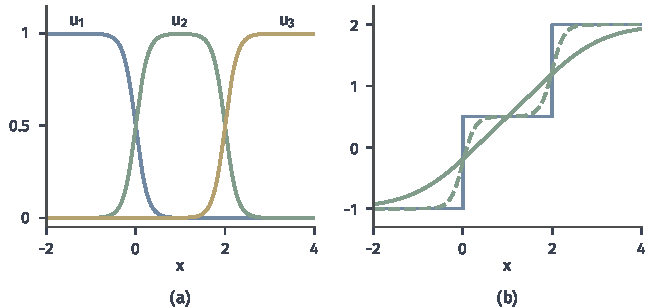
\includegraphics[width=112mm]{figures/05-optimization/03-nonsmooth-optimization/matplotlib/ns-inner-maximizer/figure.pdf}
  \caption{三段折线的熵平滑。(a)$\mu=0.2$时的内层最优权重$u_i=p_i(x)$，蓝、绿、黄分别对应斜率$-1,\tfrac12,2$的分支。(b)蓝线是原函数的次微分（台阶），绿色虚线和实线分别是$\mu=0.2$和$\mu=1$的$f_\mu'$，由权重加权平均得到。}
  \label{fig:ns-inner-maximizer}
\end{BookInlineFigure}

\paragraph{与Huber比较}
$\lvert x\rvert=\max\{x,-x\}$有两个分支，$m=2$，把两种平滑写出来：
\[
 \varphi_\mu(x)=\mu\ln\bigl(e^{x/\mu}+e^{-x/\mu}\bigr),\qquad f_\mu(x)=\mu\ln\cosh\frac{x}{\mu}.
\]

两者的导数都是$\tanh(x/\mu)$，二阶导数都不超过$1/\mu$，这与Huber函数的$1/\mu$相同。差别在形状和偏差，图~\ref{fig:ns-log-sum-exp}对比了三者（$\mu=\tfrac12$）。

\begin{BookInlineFigure}
  \centering
  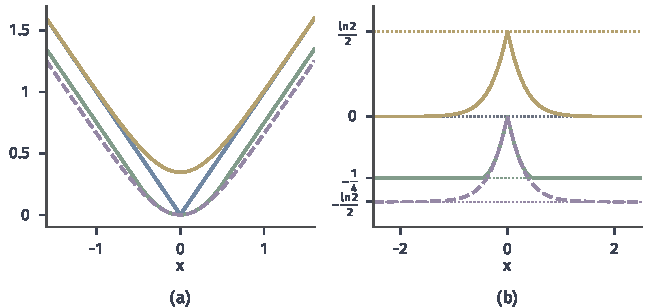
\includegraphics[width=112mm]{figures/05-optimization/03-nonsmooth-optimization/matplotlib/ns-log-sum-exp/figure.pdf}
  \caption{$\lvert x\rvert$（蓝）的三种平滑，$\mu=\tfrac12$：Huber（绿）、未平移的对数和指数函数$\varphi_\mu$（黄）、归一化版本$f_\mu$（紫色虚线）。(a)函数值。(b)替代函数减$\lvert x\rvert$的差，点线标出各自的极限或最大偏差$-\mu/2$、$\pm\mu\ln2$。}
  \label{fig:ns-log-sum-exp}
\end{BookInlineFigure}

Huber函数在$\pm\mu$外与$\lvert x\rvert$只差一个常数，偏差$\mu/2$；对数和指数函数的过渡是指数式的，走不到精确的斜率$\pm1$，偏差最大是$\mu\ln2\approx0.693\mu$。上方的$\varphi_\mu$偏差在原点最大，向外趋于零；下方的$f_\mu$在原点无偏差，向外趋于$\mu\ln2$。表~\ref{tab:ns-smoothers}汇总了这些差别。

\begin{BookInlineTable}
  \centering
  \small
  \begin{tabular}{@{}llll@{}}
    \toprule
     & Huber & 上方$\varphi_\mu$ & 下方$f_\mu$\\
    \midrule
    构造 & Moreau包络 & 负熵，不平移 & 负熵，归一化\\
    偏差范围 & $[0,\mu/2]$ & $[0,\mu\ln2]$ & $[0,\mu\ln2]$\\
    相对原函数 & 下方 & 上方 & 下方\\
    梯度Lipschitz & $1/\mu$ & $1/\mu$ & $1/\mu$\\
    二阶可微 & 否 & 是 & 是\\
    推广到$m$个分支 & 需要邻近映射 & 显式，偏差$\mu\ln m$ & 显式，偏差$\mu\ln m$\\
    \bottomrule
  \end{tabular}
  \caption{$\lvert x\rvert$的三种光滑替代。}
  \label{tab:ns-smoothers}
\end{BookInlineTable}

\subsection{平滑偏差与求解精度}
\label{sec:ns-smoothing-accuracy}

光滑化引入了两种误差：替代目标与原目标的差别，以及替代问题没有求准的部分。给定原问题的精度要求，这两者要联合分配。

\paragraph{误差分解}
设$F$是原目标，光滑替代$F_\mu$满足统一偏差界$F_\mu\leq F\leq F_\mu+\mu D$，例如式~\eqref{eq:ns-nesterov-gap}。对任意$\hat{\bm{x}}$和$F$的最小点$\bm{x}^\star$，由$F(\hat{\bm{x}})\leq F_\mu(\hat{\bm{x}})+\mu D$和$F_\mu(\bm{x}^\star)\leq F^\star$，
\begin{equation}
 F(\hat{\bm{x}})-F^\star\leq\bigl(F_\mu(\hat{\bm{x}})-F_\mu(\bm{x}^\star)\bigr)+\mu D.
 \label{eq:ns-smoothing-split}
\end{equation}

右端第一项是求解误差，可以靠多走几步减小；第二项是平滑偏差，无论替代问题解得多准都留在那里。这里的比较点取$\bm{x}^\star$而不是$F_\mu$的最小点，因此第一项可以直接用定理~\ref{thm:ns-fista-rate}的任意比较点版本控制。上方逼近的$\varphi_\mu$与$f_\mu$只差常数，上式同样适用。

图~\ref{fig:ns-smoothing-budget}(a)在$\mathbb{R}^2$上$7$个分支的问题上显示了这件事：固定$\mu$跑加速方法，原目标差最终停在由$\mu\ln m$决定的平台上；$\mu$越小，平台越低，到达平台需要的步数越多。

\begin{BookInlineFigure}
  \centering
  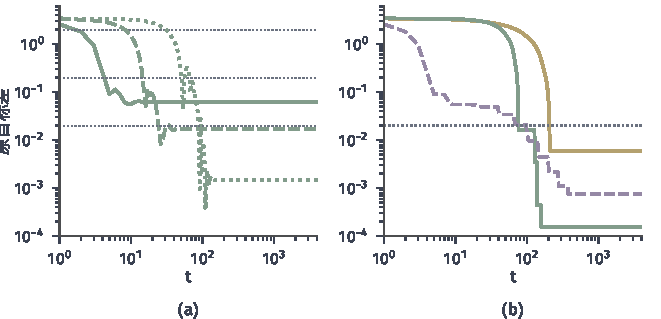
\includegraphics[width=112mm]{figures/05-optimization/03-nonsmooth-optimization/matplotlib/ns-smoothing-budget/figure.pdf}
  \caption{偏差与求解精度（双对数坐标）。目标是平面上$7$个等分方向的单位斜率分支的最大值，$\bm{x}^{(0)}=(3,2)$，用熵平滑配合Nesterov加速，$\alpha=1/L_\mu=\mu$。(a)绿色实线、虚线、点线分别是$\mu=1,0.1,0.01$时原目标差，灰色点线是偏差上界$\mu\ln7$。(b)目标精度$\varepsilon=0.02$（灰色点线）：黄线是固定步长$\alpha=\varepsilon$的次梯度法的最好值，绿线是取$\mu=\varepsilon/(2\ln7)$的平滑加速法，紫色虚线是$\mu$逐阶段减半、同步更新步长的方案。}
  \label{fig:ns-smoothing-budget}
\end{BookInlineFigure}

\paragraph{总成本}
下面的定理把偏差、光滑常数、加速方法合在一起。

\begin{theorem}[平滑加速法的总成本]
\label{thm:ns-smoothing-cost}
设$F=\psi+f$，$\psi$是凸函数且梯度$L_\psi$-Lipschitz连续（可以为零），$f$具有式~\eqref{eq:ns-max-form}的结构，$F$存在最小点$\bm{x}^\star$，$\lVert\bm{x}^{(0)}-\bm{x}^\star\rVert_2\leq R$。对$F_\mu=\psi+f_\mu$运行式~\eqref{eq:ns-fista}（$r=0$），步长$\alpha=1/L_\mu$，$L_\mu=L_\psi+\lVert\bm{A}\rVert^2/(\mu\sigma)$。给定$\varepsilon>0$，取
\begin{equation}
 \mu=\frac{\varepsilon}{2D},
 \label{eq:ns-mu-choice}
\end{equation}
则当
\begin{equation}
 T+1\geq2R\sqrt{\frac{L_\psi}{\varepsilon}}+\frac{2\sqrt{2}\,R\lVert\bm{A}\rVert}{\varepsilon}\sqrt{\frac{D}{\sigma}}
 \label{eq:ns-smoothing-iterations}
\end{equation}
时，$F(\bm{x}^{(T)})-F^\star\leq\varepsilon$。
\end{theorem}

\begin{proof}
由定理~\ref{thm:ns-nesterov}，$F_\mu$是凸函数，梯度$L_\mu$-Lipschitz连续。由定理~\ref{thm:ns-fista-rate}取$\bm{z}=\bm{x}^\star$，
\[
 F_\mu(\bm{x}^{(T)})-F_\mu(\bm{x}^\star)\leq\frac{2L_\mu R^2}{(T+1)^2}.
\]

代入式~\eqref{eq:ns-smoothing-split}，取$\mu=\varepsilon/(2D)$使偏差为$\varepsilon/2$，只需
\[
 (T+1)^2\geq\frac{4L_\mu R^2}{\varepsilon}=\frac{4R^2L_\psi}{\varepsilon}+\frac{8R^2D\lVert\bm{A}\rVert^2}{\sigma\varepsilon^2}.
\]

用$\sqrt{a+b}\leq\sqrt{a}+\sqrt{b}$开方，即得式~\eqref{eq:ns-smoothing-iterations}。
\end{proof}

第一项是光滑部分的成本，第二项$O(1/\varepsilon)$来自平滑。它比次梯度法的$O(1/\varepsilon^2)$好一个量级，代价是必须知道最大值的结构，并能求$\bm{u}_\mu$，所以这不违反黑箱下界。

用三段折线代入，$\psi=0$，$\varepsilon=0.1$，$D=\ln3$，$\max_i a_i^2=4$，$\sigma=1$，初始距离$R=4$。先算平滑参数和光滑常数，
\[
 \mu=\frac{0.1}{2\ln3}\approx0.0455,\qquad L_\mu=\frac{4}{\mu}\approx87.9.
\]

代入定理，步数上界为
\[
 T+1\geq2R\sqrt{L_\mu/\varepsilon}\approx237.
\]

次梯度法的上界$R^2G^2/\varepsilon^2=16\cdot4/0.01=6400$，这是相对同一个$\varepsilon$的比较。

\paragraph{联合选参数}
式~\eqref{eq:ns-smoothing-split}说明步长、平滑参数和停止阈值都不能单独选。$\mu$减小时偏差变小，$L_\mu$变大，步长$1/L_\mu$变小。停止阈值设得比$\mu D$小很多没有意义，因为剩下的误差由偏差主宰；设得比$\mu D$大，又浪费了平滑的精度。上面的取法$\mu D=\varepsilon/2$就是让两者各占一半。

固定一个很小的$\mu$从头跑，前期$L_\mu$大、步长小，推进很慢。实践中常用逐阶段减小$\mu$的办法：先用大的$\mu$求解，把结果作为下一阶段的起点，$\mu$减半，直到目标值。这时有两点必须同步：每一次改变$\mu$，步长必须按新的$L_\mu$更新，否则旧步长可能超过$1/L_\mu$，上一节的一步不等式不再成立；外推参数$\theta$也要重置，因为不同阶段实际上是不同的目标函数。

图~\ref{fig:ns-smoothing-budget}(b)中，逐阶段的方案（紫色虚线）前几十步明显领先；三种方法达到$\varepsilon=0.02$所用的步数分别约为次梯度法$207$、固定小$\mu$的加速法$76$、逐阶段方案$98$。这个小例子上后两者相差不大，差别主要在前期，具体的阶段长度也会影响结果。

\paragraph{替代目标下降不代表原目标下降}
梯度方法在$F_\mu$上下降，原目标却可能上升。用三段折线，$\mu=1$，$\alpha=\mu/4$，从原问题的最优解$x^{(0)}=0$出发，由前面算出的$f_1'(0)\approx-0.195$，
\[
 x^{(1)}\approx0.049.
\]

原目标从最小值$0$升到约$0.024$，替代目标（归一化版本）则从约$-0.381$降到约$-0.390$。图~\ref{fig:ns-surrogate-rise}是这一过程的全貌：替代问题的最小点不在原问题的解上，迭代朝前者走，原目标一路上升到某个水平。这个上升不超过偏差上界。

\begin{BookInlineFigure}
  \centering
  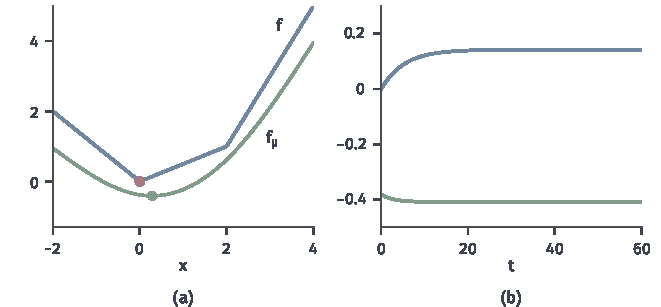
\includegraphics[width=112mm]{figures/05-optimization/03-nonsmooth-optimization/matplotlib/ns-surrogate-rise/figure.pdf}
  \caption{替代目标下降时原目标可以上升。三段折线，$\mu=1$，$\alpha=\tfrac14$，从原问题的解（红点）出发。(a)蓝线是$f$，绿线是$f_\mu$，绿点是$f_\mu$的最小点。(b)蓝线是原目标值，单调上升到平台；绿线是替代目标值，单调下降。}
  \label{fig:ns-surrogate-rise}
\end{BookInlineFigure}

所以光滑化方法要同时记录原目标值，并由式~\eqref{eq:ns-smoothing-split}判断最终结果。这是光滑化与邻近方法的一个重要差别：邻近方法每轮都直接面对原目标$F$。
